\subsubsection{Mount interface}
Rotator is designed to be mounted on tripod and can be deployed outdoors. To fulfil this requirement a standard mount is designed which can provide mechanical joint between differential shaft of rotator and tripod rod as shown in following figure 400.8.  
\begin{figure}[H]
	\centering
	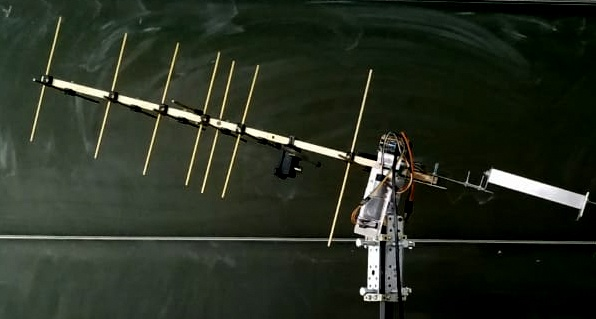
\includegraphics[width=\linewidth]{../art/real image.jpeg}
	\caption{Mount Prototype}
\end{figure}

\subsubsection*{Mount interface design methodology}
Design of mount is inspired from lathe chuck which has mechanism to hold any work-piece. In this design similar capability is achieved by providing 8 nut bolts which can hold tripod of 10 mm to 40 mm diameter. Further this design has capability to compensate levelling of rotator with respect to horizon by 10 deg. on each side. Following figure shows mount and it’s connection differential gear.   

\begin{figure}[H]
	\centering
	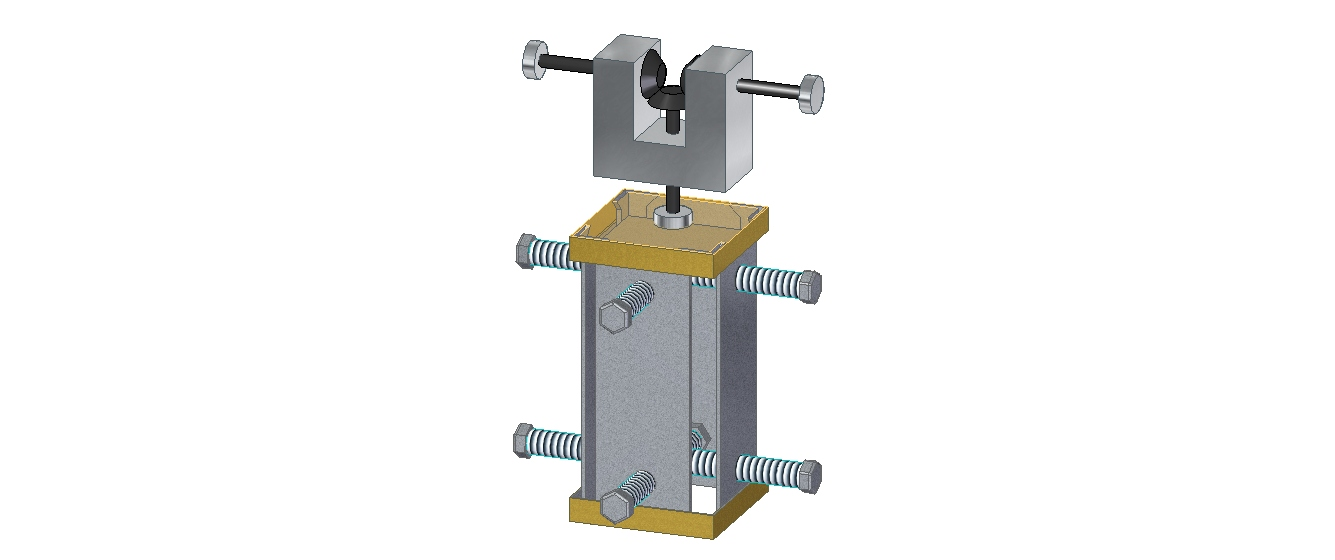
\includegraphics[width=0.9\linewidth]{../art/m.jpg}
	\caption{Mount image CAD}
\end{figure}

\subsubsection*{Scope of improvements}
Other mounting options can be explored to reduce the cost and complexity of the design. These improvement can be implemented by using off the shelf technologies. One of the option is usage of sound box adaptor for mount as shown in figure 400.10.     

\begin{figure}[H]
	\centering
	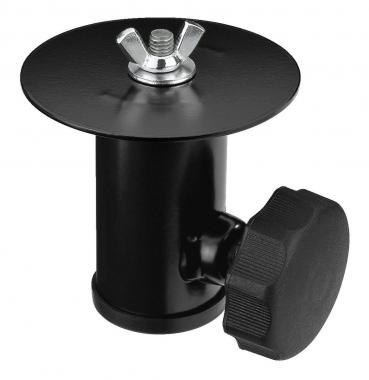
\includegraphics[width=0.2\linewidth]{../art/buy mount.jpg}
	\caption{Example of off shelf technology}
\end{figure}